\section{Testing and Evaluation}
\subsection{Overview}
The previous chapter guided as through the implementation of the design of our system and also presented the framework on which our system was implemented. In this chapter we will look at the methods used to evaluate our system. We will discuss how well our system addressed the issue it was set out to address and how it performed in the tests used in the evaluation.
\subsection{Methodology}
This section presents the methods used in testing the functionalities and features of our system and how well our system performed under each method.
\subsubsection{Browser Tests}
A web browser \footnote{A software to display HTML and interpret JavaScript} was used in evaluating our system as our system operates in a browser setting. There are several web browsers and our system needs to behave in a consistent manner across all the browser platforms. Our system uses some experimental features that are not implemented on all browsers yet, due to this the browser test was predominantly performed on google chrome. \cite{website:GoogleChrome}
The figure \ref{fig:homeScreen} below shows how google chrome rendered our system's UI.
\begin{figure}[!ht]
\caption{Google Chrome : Rendering of our system's home Screen}
    \label{fig:homeScreen}
    \centering
    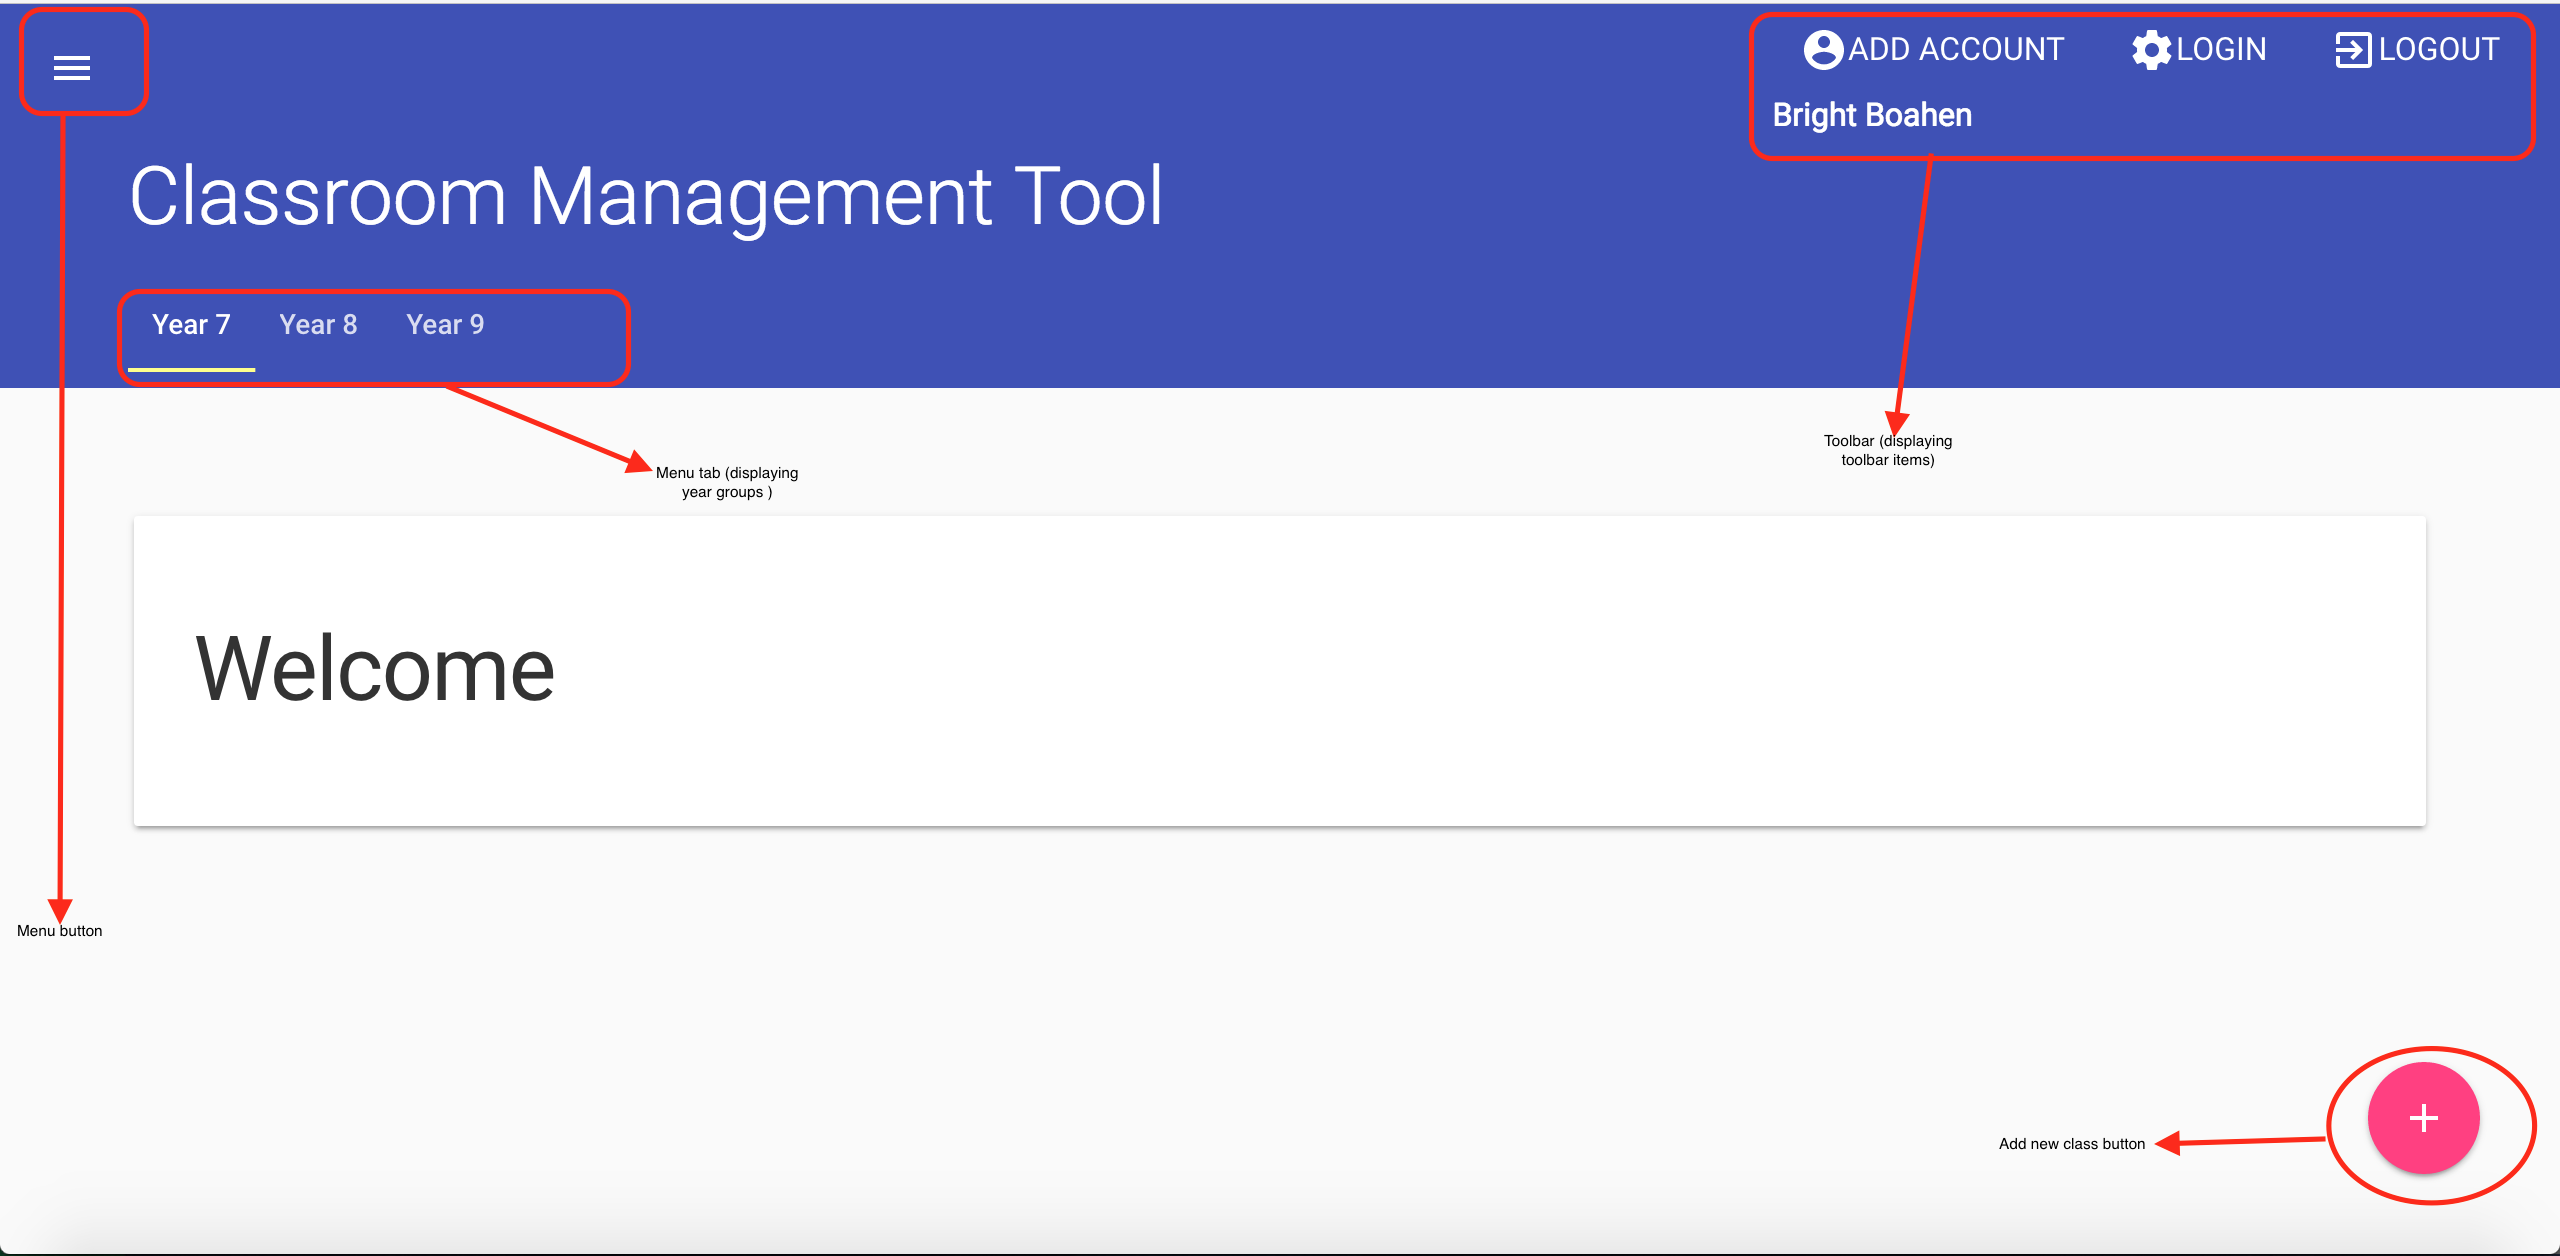
\includegraphics[scale=0.3]{figures/home_screen}
\end{figure}
Figure \ref{fig:homeScreen} above is annotated the UI components that were expected to be on diplay on the home screen. These are :
\begin{itemize}
    \item menu button -  on the top left corner,
    \item toolbar - on the top right corner,
    \item menu tabs - below the menu button, 
    \item Add new button - bottom right corner
\end{itemize}
Figure \ref{fig:canvas} below illustrates the result of our system's classroom component in a web browser \cite{website:GoogleChrome}.
\begin{figure}[!ht]
    \caption{Google Chrome : Rendering of the classroom}
    \label{fig:canvas}
    \centering
    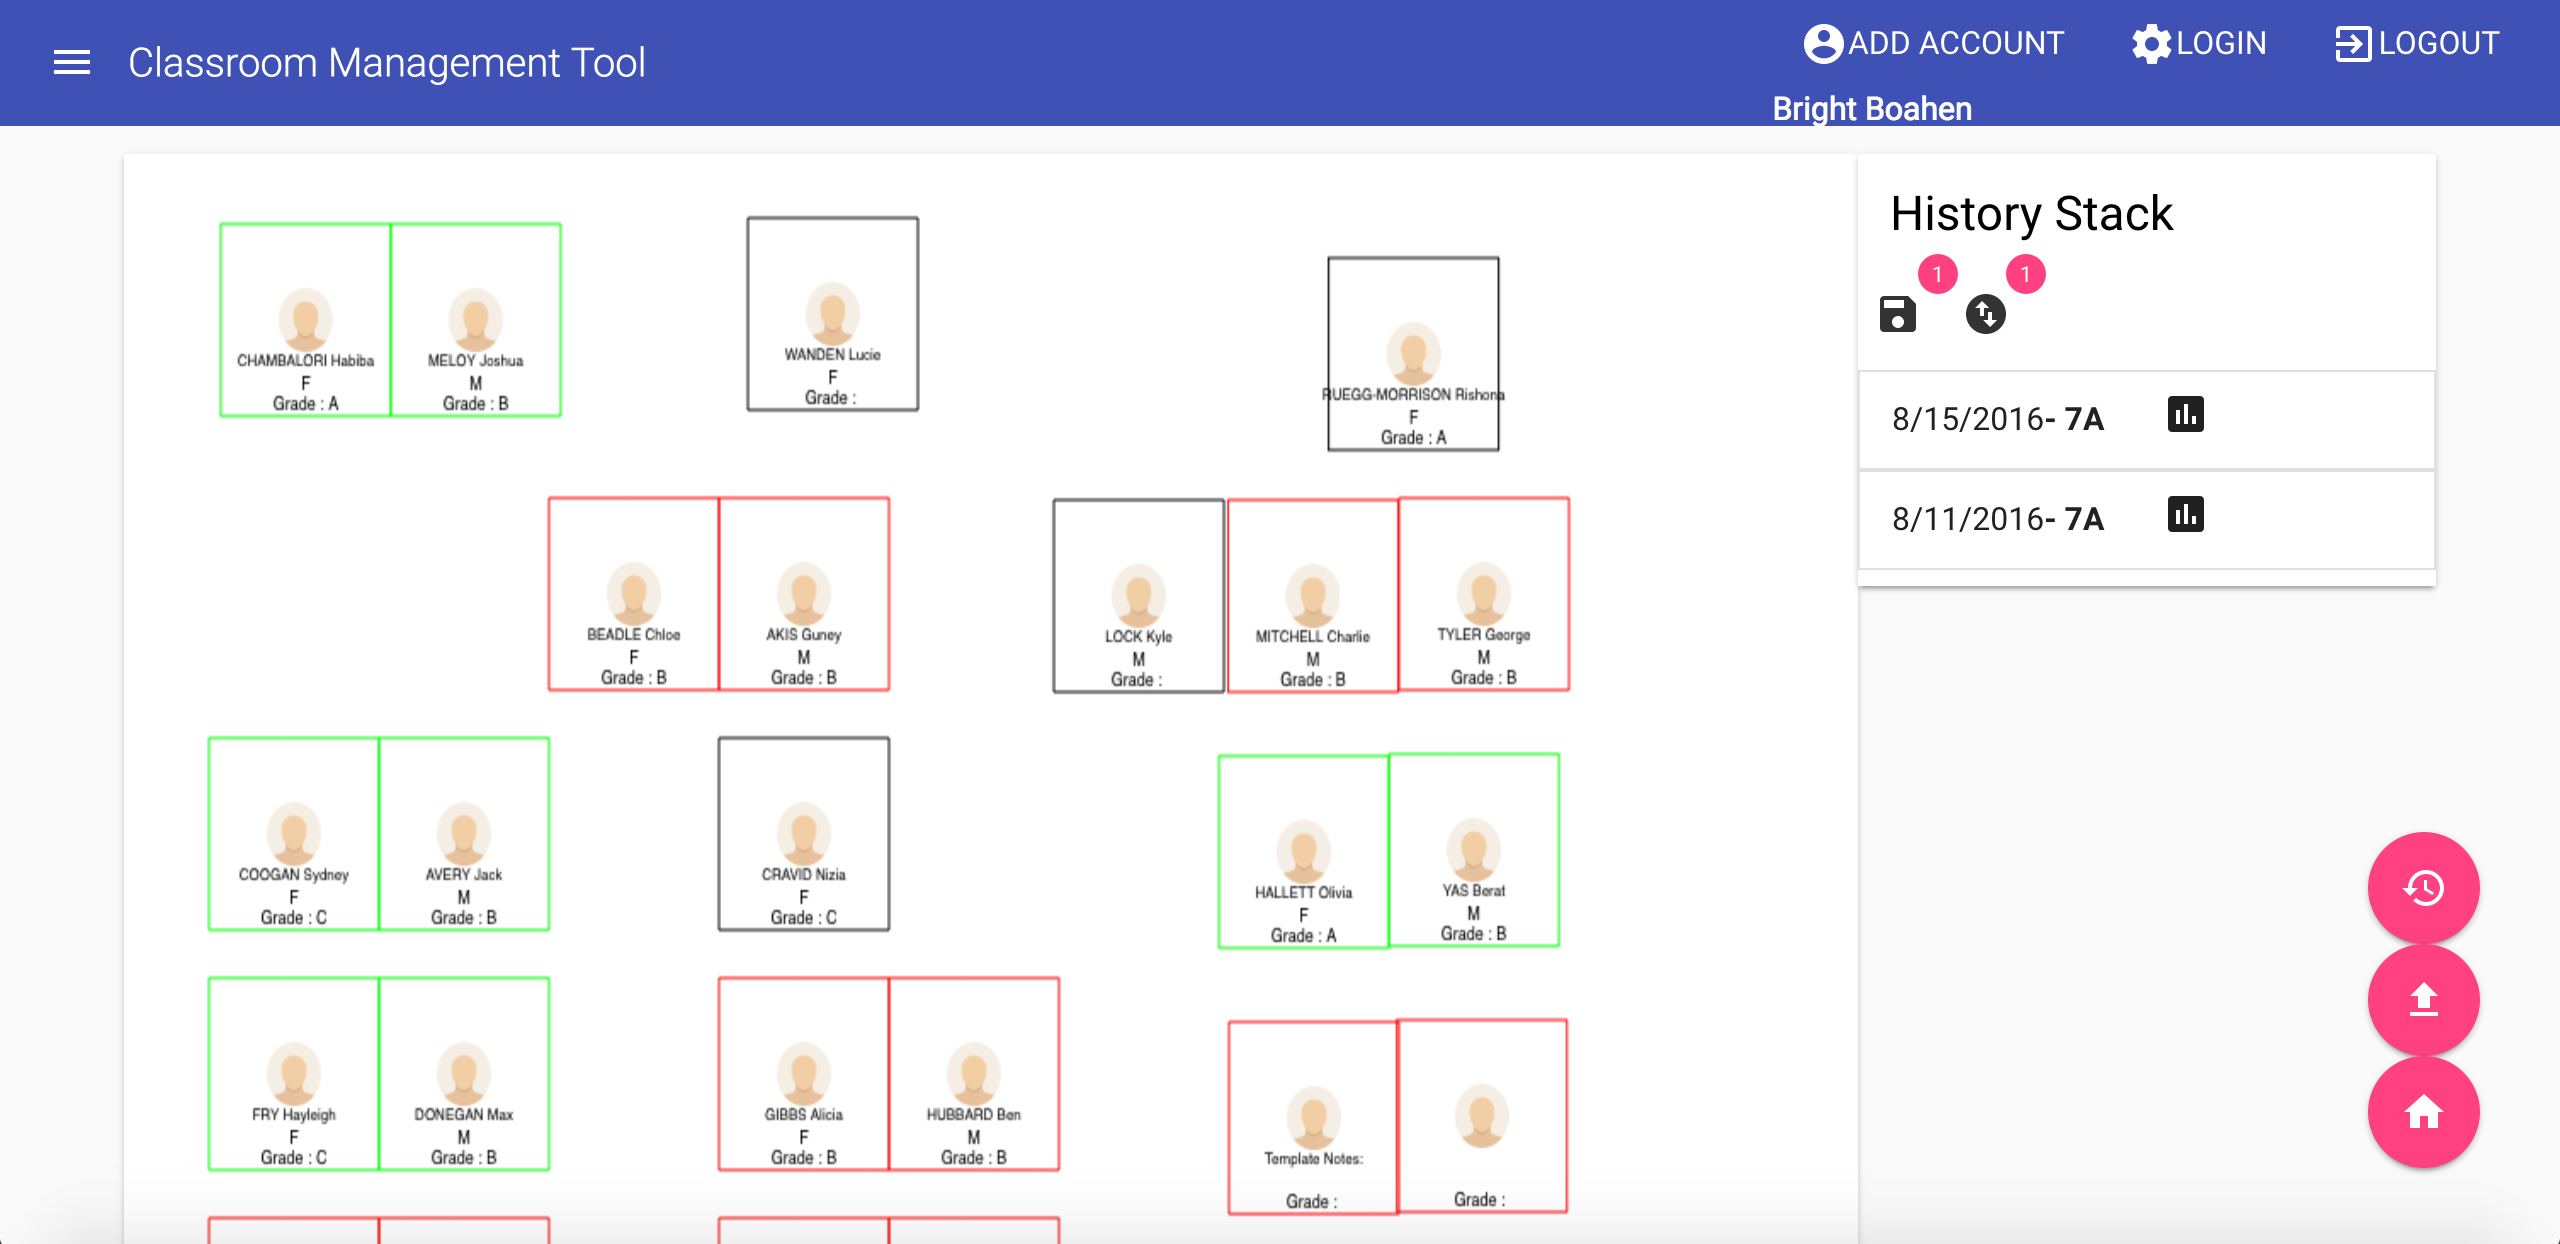
\includegraphics[scale=0.3]{figures/classroom}
\end{figure}
In figure \ref{fig:canvas} above we can see the \emph{History Manager} rendered clearly on the right side with some previous seating arrangements. To the left of the \emph{History Manager} is the \emph{classroom canvas}. The result is as expected as the rule has been applied and optimal pairings coloured ``green'' and worst pairings or groups coloured ``red''.

\subsubsection{Unit Tests}
Unit testing is the process of testing individual units(components) or groups of related units. \cite{runeson2006survey}. Our system is made of several units that together compose the system. It was necessary to test these units to ensure they perform their responsibilities effectively and efficiently.

We use Web Component Tester(WCT) \cite{website:Polymer-Github} to test our components. WCT provides a browser based environment for us to test our components.
\begin{table}
    \begin{tabular}{|c|c|}
        \hline
        \multicolumn{2}{|c|}{Unit Tests on Google Chrome} \\
        \hline
        Unit(component)         &     Test Result \\
        \hline
        Classroom canvas        &     Passed \\
        HistoryStack            &     Passed \\
        MenuTab                 &     Passed \\
        Toolbar                 &     Passed \\
        \hline
    \end{tabular}
    \caption{\label{tab:unit-chrome}Unit tests performed on core components of our system in google chrome browser.}
\end{table}

\begin{table}
    \begin{tabular}{|c|c|}
        \hline
        \multicolumn{2}{|c|}{Unit Tests on Internet Explorer} \\
        \hline
        Unit(component)         &     Test Result \\
        \hline
        Classroom canvas        &     Passed \\
        HistoryStack            &     Failed \\
        MenuTab                 &     Passed \\
        Toolbar                 &     Failed \\
        \hline
    \end{tabular}
    \caption{\label{tab:unit-explorer}Unit tests performed on core components of our system on internet explorer browser.}
\end{table}
As we can see from table \ref{tab:unit-chrome} the critical components passed on the unit tests but on Internet Explorer (alternate web browser) two of the components failed due to some experimental web features that are not fully supported by Internet Explorer.
\subsubsection{User Tests} \label{sub:user-testing}
In \ref{sub:userRequirments} section we discussed the features and functionalities expected of our system by the user. With this in mind we conducted a ``black box'' testing with users by asking potential serious \footnote{ serious user refers to a teacher} users who have no prior knowledge of the system to use the system and we evaluated their response on the clarity of use and whether they used less cognitive skills when performing their seating tasks.
\begin{table}
    \begin{tabular}{|c|c|c|c|c|}
        \hline
        \multicolumn{5}{|c|}{User Testing} \\
        \hline
        Age & Sex & Subject & Clarity & Level of cognition \\
        \hline
        30  & Female & Drama & 3 out of 5 & 4 out 5\\
        \hline
    \end{tabular}
    \caption{\label{tab:user-testing1} Black box testing with users - first round}
\end{table}


Table \ref{tab:user-testing1} illustrates the response of the user after her first encounter with our system.
\begin{table}
    \begin{tabular}{|c|c|c|c|c|}
        \hline
        \multicolumn{5}{|c|}{User Testing} \\
        \hline
        Age & Sex & Subject & Clarity & Level of cognition \\
        \hline
        30  & Female & Drama & 4 out of 5 & 2 out 5\\
        \hline
    \end{tabular}
    \caption{\label{tab:user-testing2} Black box testing with users - second round}
\end{table}


Table \ref{tab:user-testing2} illustrates the response of the user after her second encounter with our system.

From tables \ref{tab:user-testing1} and \ref{tab:user-testing2} we can see that the users perception of our system improved, that is she found it more clear the second time although the level of clarity was average the first time and the level of cognition( that is the thinking she had to do) also reduced dramatically on her second attempt. 
\subsubsection{Remarks on tests}
We based based the user tests in  \ref{sub:user-testing} on two main concepts.
\begin{itemize}
    \item Clarity,
    \item Cognitive Skills.
\end{itemize}
This is because we can use these two as a metric to judge the system whether it meets all the user requirements mentioned in \ref{sub:userRequirments} . Clarity involves all the steps of the use while performing their tasks in the system and cognitive skills involves how hard they have had to think about their tasks. A high cognitive value would indicate the system is not achieving its adaptivity requirement and if they steps are not clear enough the user cannot perform their tasks. The system fails its overall aim.

The result from the tests in \ref{tab:user-testing1} and \ref{tab:user-testing2} cannot be conclusive as we were only able to get one serious user to undertake the test. It may not be conclusive but it gave us an indication of the potential of the system in achieving its goals. We also could not conduct real time test by asking teachers to use the system for a class and report on how well the seatings recommended by the system performed.
\subsection{Summary}
In this chapter we have presented evidence of how well our system achieves its aims and objectives. We have seen how the individual components performed and how the overall system meets the requirement of a user.